% Chapter Template

\chapter{Work Procedure} % Main chapter title

\label{Chapter4} % Change X to a consecutive number; for referencing this chapter elsewhere, use \ref{ChapterX}

\lhead{Chapter 4. \emph{Work Procedure}} % Change X to a consecutive number; this is for the header on each page - perhaps a shortened title

%----------------------------------------------------------------------------------------
%	SECTION 1
%----------------------------------------------------------------------------------------
The aim of the this project is to detect the MW phase of mind more precisely with lowest false alarm. A set of steps have been followed to complete the procedure. A diagram has been given to illustrate in Figure ~\ref{fig:work_procedure} with a comprehensive description given in section. Data pre-processing,Normalization feature extraction, and classification are the basic steps to train a model and classify the MW phase.


\begin{figure}
    \centering
    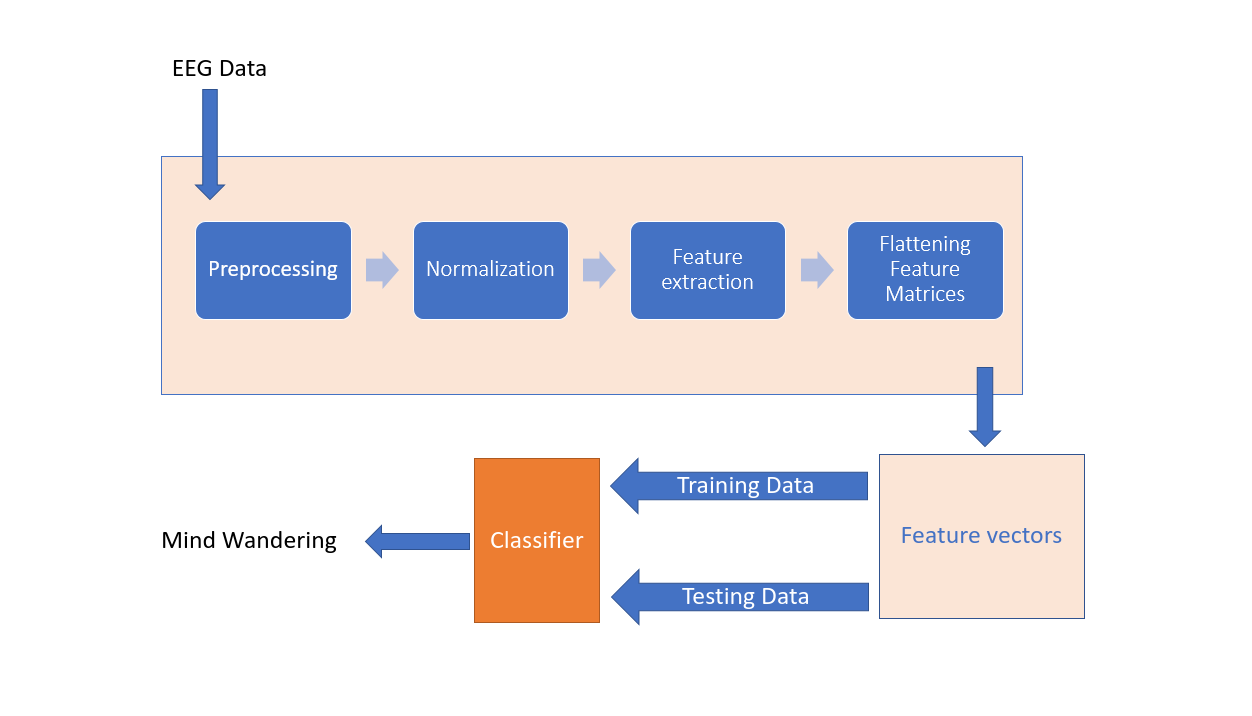
\includegraphics[width=15cm]{Pictures/workprocedure.png}
    \caption{Work Procedure }
    \label{fig:work_procedure}
\end{figure}

\section{Data Pre-processing}

Data was recorded from 64 channels with 1024 Hz sampling rate.By comparing source  activation levels,a significant change in the power of the  $\theta$- and $\alpha$ band observed in the MPC, the PCC, and the temporo-parietal junction (In MTP-I). So,we focused on the $\theta$ band (3.5Hz-7Hz) and $\alpha$ -band (8-16 Hz) in our study.We limit our study to  $\alpha$ and $\theta$  frequency bands that is 3–16 Hz. The lower $\theta$ band frequency boundary was set to 3 Hz for both subjects, while the upper $\alpha$ band frequency boundary was set to 16 Hz. Then all the questionnaire sessions were removed from the data. Channel signals containing  electrical and eye blink artifacts (as assessed by visual inspection) or high frequency noise were removed and clean data set reformed. Then the signal was converted to average reference level .Lastly , data set was normalized for data mining.
 
\begin{figure}
    \centering
    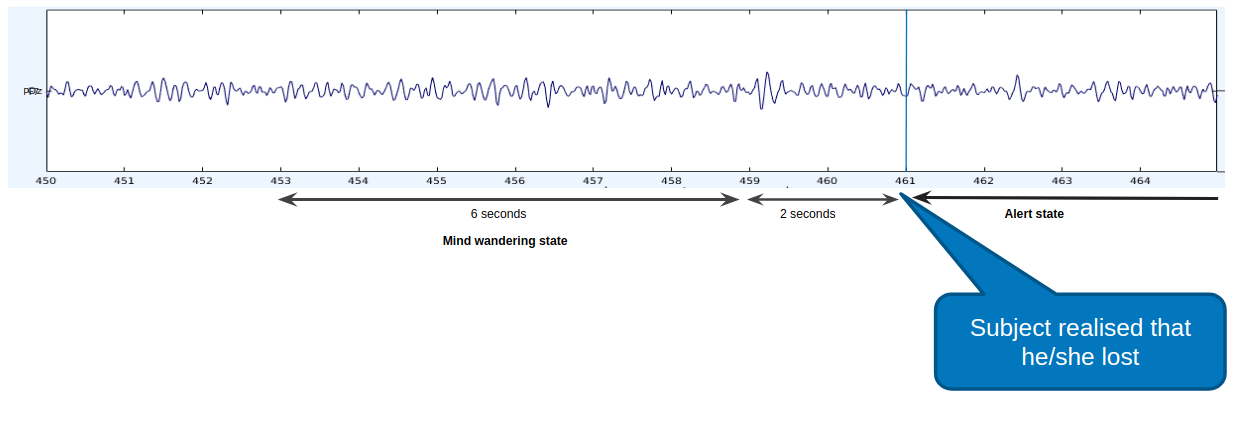
\includegraphics[width=15cm]{Pictures/single_chanel_data.png}
    \caption{Button press event,Alertness and Mind wandering}
    \label{fig:Mw_fig}
\end{figure}

\subsection{Alertness and MW data extraction}
 The data was collected continuously.So, it was contaminated with alertness data.During the data collection subjects had to press button when they realized that they were lost.So, we considered that it took 2 seconds of time to realize and press the button.And we also considered that subject was in mind-wandering state at least for 4 seconds.For mind-wandering data, we extracted data from -6 to -2 seconds as MW state and 2 to 6 seconds as alertness state where button press event occured at 0 second.All the events and time laps illustrated in Figure ~\ref{fig:Mw_fig}.
 
As a result of above procedure, we got 977 files containing a 2D matrix each correspond to either MW or Alertness.A row contains data of a channel collected in 4 seconds that is 4X1024 samples.There were 64 channels and each channel has 4096 readings.Each 2D matrix has dimension of 64 X 4096.   

\section{Normalization}
The Z-score normalization method has been used to normalize the EEG samples collected during breath counting task. Samples were normalized to have a standard deviation of 1 and a zero mean . The dimension of our dataset is [977,64,8192](total sample,\# channels,total time instances). It means there are 977 samples of dimension [64,8192] each. So mean and standard deviation were calculated for all signals. We normalized the  training samples by subtracting the mean and dividing the result by standard deviation.The standard deviation and Mean of training set have been stored in a file to later normalize the testing and validation set.

\section{Feature extraction}
To reduce the dimension we used feature extraction method.In the process of feature extraction,the relevant information to perform a desired task is expected to keep,instead of keeping complete information.Our data-set consist of 19 sessions containing specific task related to our investigation. This sessions was acquired from two subjects. Then we used built in methods of MATLAB and various Python libraries to extract features, which are mentioned below:


\begin{itemize}
    \item Coefficient of variation
    \item first difference
    \item slope mean
    \item slope variance
    \item kurtosis
    \item second difference mean
    \item second difference max
    \item skewness
    \item first difference mean
    \item first difference max
    \item fractal dimension
    \item Auto regressive model parameters 
    \item Hjorth parameters
    \item wavelet features
    
\end{itemize}
\subsection{Coefficient of variation}
The statistical measure of the dispersion of date instances  around the mean a data set is called coefficient of variation (COV) . The coefficient of variation represented by the ratio of standard deviation to the mean. And the usefulness of COV statistic is to compare the degree of variation two data series , even if they have drastically different means .
\begin{equation}
 \label{coeff_var}
 \begin{split}
    C_v = \frac{\sigma}{\mu}  
 \end{split}
\end{equation}

Where :
$$\sigma = Standard Deviation  $$
$$\mu = mean$$

\subsection{First Difference}
First difference is an array containing difference of previous element with the current element.
\begin{lstlisting}[language=Python]
def first_diff(i):
    b=i
    out = np.zeros(len(b))
    for j in range(len(i)):
        out[j] = b[j-1]-b[j]# Obtaining the 1st Diffs
        j=j+1
        c=out[1:len(out)]
    return c #returns first diff
\end{lstlisting}

\subsection{slope mean}
First we calculated slopes of each row using maximum and minimum amplitude, then we took mean of all slopes. 
\subsection{slope variance}
We calculated slope using above method then we calculated variance of slopes.  
\subsection{Skewness}
The measure of the distortion degree from  the normal distribution or the symmetrical bell curve, is the Skewness. It measures the feeble amount of balance of parts, same on 2 sides in data distribution.Zero Skewness indicates a symmetrical distribution.\\
Figure \ref{fig:skewness} shows the Skewness result of our subject 1 task 1 in .
\\
Types of Skewness: Negative and Positive\\
 The  right side tail of the distribution is quite longer or fatter than the left side tail in positive skewness. The mode will have lesser value than mean and median.\\
 The  right side tail of the distribution is quite smaller or thinner than the left side tail in negative skewness. The mode will have greater value than mean and median.
\begin{figure}
    \centering
    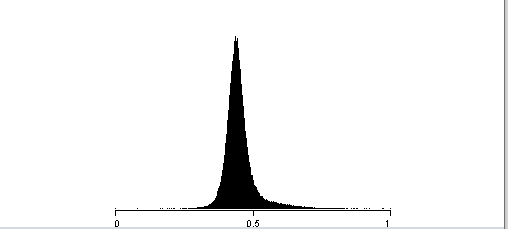
\includegraphics[width=15cm]{Pictures/skewness.png}
    \caption{Skewness result}
    \label{fig:skewness}
\end{figure}
\subsection{Kurtosis}
Kurtosis is the measure of the tails of the distribution,it is not about the  flatness or the peakedness.  To outline the uttermost values in one vs the other tail,kurtosis has been used.Basically  Kurtosis is the measure of outliers  of the distribution.We have shown the sample Kurtosis graph,in the Figure \ref{fig:kurtosis} .
\begin{figure}
    \centering
    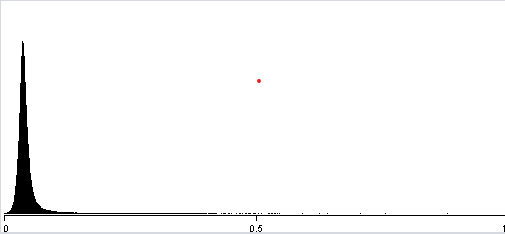
\includegraphics[width=15cm]{Pictures/kurtosis.png}
    \caption{Kurtosis:sample diagram}
    \label{fig:kurtosis}
\end{figure}
\subsection{First difference mean}
First difference mean is the average of  first difference of an array.where,First difference is an array containing difference of previous element with the current element.
\begin{lstlisting}[language=Python]
def first_diff_mean(arr):
    data = arr 
    diff_mean_array = np.zeros(len(data)) #Initialinling the array as all 0s
    index = 0; #current cell position in the output array
    for i in data:
        sum=0.0#initializing the sum at the start of each iteration
        for j in range(len(i)-1):
            sum += abs(i[j+1]-i[j]) # Obtaining the 1st Diffs
        diff_mean_array[index]=sum/(len(i)-1)
        index+=1 #updating the cell position
    return np.sum(diff_mean_array)/1
\end{lstlisting}

\subsection{First difference max}
First difference max is the maximum value in first difference array.where,First difference is an array containing difference of previous element with the current element.
\begin{lstlisting}[language=Python]
def first_diff_max(arr):
    data = arr 
    diff_max_array = np.zeros(len(data)) #Initialinling the array as all 0s
    first_diff = np.zeros(len(data[0])-1)#Initialinling the array as all 0s 
    index = 0; #current cell position in the output array
    for i in data:
        max=0.0#initializing at the start of each iteration
        for j in range(len(i)-1):
            first_diff[j] = abs(i[j+1]-i[j]) # Obtaining the 1st Diffs
            if first_diff[j]>max: 
                max=first_diff[j] # finding the maximum of the first differences
        diff_max_array[index]=max
        index+=1 #updating the cell position
    return np.sum(diff_max_array)/1
\end{lstlisting}

\subsection{Fractal dimension (FD)}
The entropy measures the randomness of a dataset.The information in a data depends on entropy. Fractal dimension is related with the entropy \cite{Boostani_2004}.Thus, from fractal dimension we can interpret the degree of  signal irregularity or signal roughness . There are two famous methods to calculate fractal dimension,that are Peterson, Katz and Higuchi methods. the Katz method has  more  robustness[11] than others, and that is why we have used this in our project. Katz methods can derives from waveform directly. The  fractal dimension curve is defined as:
$$
FD = \frac{\log_{10} L}{\log_{10} d}
$$

here,\\
$L$ : curve length \\
and \\
$d$ : diameter \\
The diameter of curve is the distance between the farthest point of the curve and the  first point of sequence. \cite{Boostani_2004}.


\subsection{Auto regressive model parameters}
We have used the whitening lattice-filter method of Burg  to calculate the coefficients of an auto-regressive (AR) model of complex data (say x) \cite{burg1968new}. The inverse of the model is a moving-average filter which reduces x to white noise. The power spectrum of the AR model is an estimate of the maximum entropy power spectrum of the data \cite{burg1968new}.

\subsection{Hjorth parameters}

These parameters elaborates the  characteristics of signal. The measure of mean frequency, deviation from sin shape and variance of signal are used to describe the  characteristics of the signal.These terms are usually called activity, mobility and complexity respectively and  are  described as follows :
$$
Activity(x)=\frac{\sum^N_{i=1} (x(i) - \mu)^2}{N}
$$
$$
Mobility = \sqrt{\frac{VAR(x')}{VAR(x)}}
$$
$$
Complexity = \frac{Mobility(x')}{Mobility(x)}
$$

where,\\
$x$ : signal, \\
$x'$: signal derivative , \\
$N $:  \# samples  \\
$\mu$ : mean of signal\\
The  window  of calculation,we have used  for these parameters is  of size 500 ms without any overlapping.


\subsection{Wavelet features}
We have calculated mean,standard deviation,energy,entropy etc. with approximation coefficients and details coefficients for each channel. The minimum, maximum and mean of all these factors make a total of 24 features which contribute in the classification of MW.
\section{Flattening Feature Matrices}
We got 52 features for each channel signal.At the end we got 2D matrices with 64 $\times$ 52  (each row contains features of a  channel).The general form of a feature vector shown below:
\begin{align*}
&\boldsymbol{ch_1:} &f_1^1&,&f_1^2&,&f_1^3 &......    &f_1^{52} \\
&\boldsymbol{ch_2:} &f_2^1&,&f_2^2&,&f_2^3 &......   &f_2^{52} \\
&  \boldsymbol{.}       &.   &,  &. &, &.    &......   &.      \\
&  \boldsymbol{.}       &.   &,  &. &, &.    &......   &.      \\
&  \boldsymbol{.}       &.   &,  &. &, &.    &......   &.   \\
&\boldsymbol{ch_{64}:} &f_{64}^1&,&f_{64}^2&,&f_{64}^3 &......&f_{64}^{52} \\
\end{align*}

$\boldsymbol{ch_i :}$ feature  vector generated from the $i^{th}$ channel signal \\
$\boldsymbol{f_q^p :}$ $p^{th}$ feature of $q^{th}$ channel signal

Instead of using the 2-dimensional features vector to train machine learning models we have flattened them in to 1D vector.To flatten them we concatenated the each row into it's previous row except the first one.Thus,feature vector got flattened without loosing any information.we saved the reference of locality. 
The resulting in feature vector shown below:
\begin{align*}
    &\boldsymbol{Flattened \; feature \; vector:} &ch_1&,&ch_2&,&ch_3 &...... &ch_{64}
\end{align*}
$$or$$
\begin{align*}
&\boldsymbol{Flattened \; feature \; vector:} &f_1^1&,&f_1^2&,&f_1^3 &......    &f_1^{52}......&f_{64}^{52} \\
\end{align*}
The meaning of all symbols are same as defined above.

At the end of each row we have concatenated the label of each matrix as it was (1 for MW and 0 for Alertness state)
\section{Models}

MW detection has no standard method to interpret the result. That is why machine learning approach is suitable to examine the dataset and apply an algorithm. In order to detect the mind wandering we classified the data using different models for all the features. Using different classifiers gave us the opportunity to measure the highest accuracy label. Classification accuracy not only depends on the classifier but also the input EEG signal. We have scrutinized our data using 1024 hz frequency rate. We differentiate the result using binary value where 1 defines MW and 0 considers focusing time.The different machine learning models we have used are described below one by one.


\subsection{Adaptive Boosting}
Yoav Freund and Robert Schapire in 1996  proposed a combination boosting classifier  known as  Adaptive Boosting or Ada-Boost classifier  \cite{freund1996experiments}. By the combination of multiple classifiers they achieved an increased  accuracy of classifiers. Ada-Boost is an iterative ensemble method. Ada-Boost algorithm combines multiple poor performing classifiers to build a strong classifier so that you will get increased accuracy strong classifier  \cite{freund1996experiments}. The core concept  of Ada-boost is to learn the weights of poor performing classifiers. And in each iteration of the training it updates the weights  such that it ensures the accurate predictions of new observations. Any machine learning model which accepts weights on the training set can be used as base classifier. Ada-boost should meet two conditions:
\begin{enumerate}
    \item The various weighed of classifier should be trained interactively on  training examples \cite{freund1996experiments}.
    \item By minimizing training error,it tries to provide an excellent fit for these examples in each iteration.  \cite{freund1996experiments}.
\end{enumerate}

 A particular method of training a boosted classifier has been used as Ada-Boost algorithm. The general form of a boost classifier is :
\begin{equation}
F_T (x) = \sum_{t=1}^T  f_t(x) 
\end{equation}
where,\\
$f_{t}$ : a weak learner that takes an object $x$ as input and returns a value that identifies the  object class.


\subsection{Support vector machine}
% The objective of the classifier is to classify the disorganized EEG signals to organized and labelled data using machine learning approach. The drawback of our dataset is that it was not mapped and the real challenge is to labeling it precisely to get the best outcome from the classifier. The classifier is a non-linear SVM where it uses a function that transforms our data in high dimensional space. It is hard to obtain a result accurately where the data in not linearly separated in high dimensional space. Achieving an unbiased classification result, the data is divided in training and testing set with the help of K-fold cross validation technique. Lastly, we have achieved accuracy for both classifier which is explained in the result and discussion part.
Support vector machine (SVM)  uses a classification algorithms for two-class classification problems.It is a supervised machine learning algorithm. After training a SVM model on a set of labeled data, it would be able to categorize them.

\begin{figure}[ht]
    \centering
    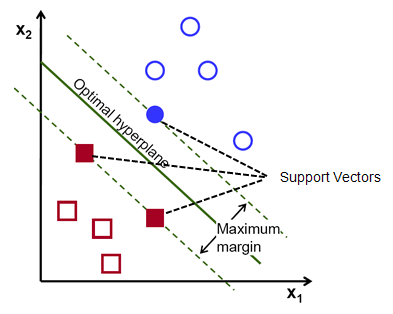
\includegraphics{Pictures/SVM_margin.png}
    \caption{SVM for a linearly classifiable input}
    \label{fig:svm}
\end{figure}
In Figure \ref{fig:svm}, you can see a SVM classifier for a linearly classifiable data.

Now a days,Support Vector Machine (SVM) classifiers is quite popular in the field of classification,regression analysis and novelty detection  in recent years,  \cite{bishop2006pattern} \cite{xie2008research}.In EEG classifiers, it has been seen that SVM gave very promising results  \cite{lal2004support}. A kernel-based algorithm has been use in Support Vector Machine to give sparse solutions.Support Vector Machine is a computationally efficient method for solving high dimensional  and complex problems, because a  kernel solution required  only for a specific subset of the training data ,not for  the entire training set.  The Support Vector Machine converges to a single minimum and also good in classification of  nonlinear data, and it makes SVM preferable to  neural network or linear  classifiers. A hyper-plane or set of hyper-planes (in a high- or infinite-dimensional space) has been constructed in SVM, which is used for  regression, classification,or other tasks e.g. outliers detection. Intuitively, a hyper-plane is a  good separator of two class.It has the highest length of project to the nearest training-data point of any class.It is also called functional margin.The  margin is inversely proportional to  the generalization error of the classifier  \cite{bishop2006pattern}:

\begin{equation}
    y(x)=w^T\varphi(x)+b 
\end{equation}

\subsection{Decision Tree}
A decision tree a method which is used for regression and classification with no hyper-parameters.It is a supervised learning method.It is a tree like structure, where node denotes feature to be tested and branches can be chose on the basis of that feature value. 

While learning a decision tree,based on a feature value, test we split the source set into subsets.We repeat this process on each derived sub-tree in a recursive manner,this is called recursive partitioning.When the subset at a node have all same value target variable or no value can be added in the prediction by further splitting, we stop the recursion. The construction of DT classifier does not require any  domain specific knowledge or any parameter setting, and therefore for exploratory knowledge discovery, it is appropriated .The higher dimensional data can be utilized while learning a decision trees. In general, we can get a good accuracy with decision tree classifier.


\begin{figure}[ht]
    \centering
    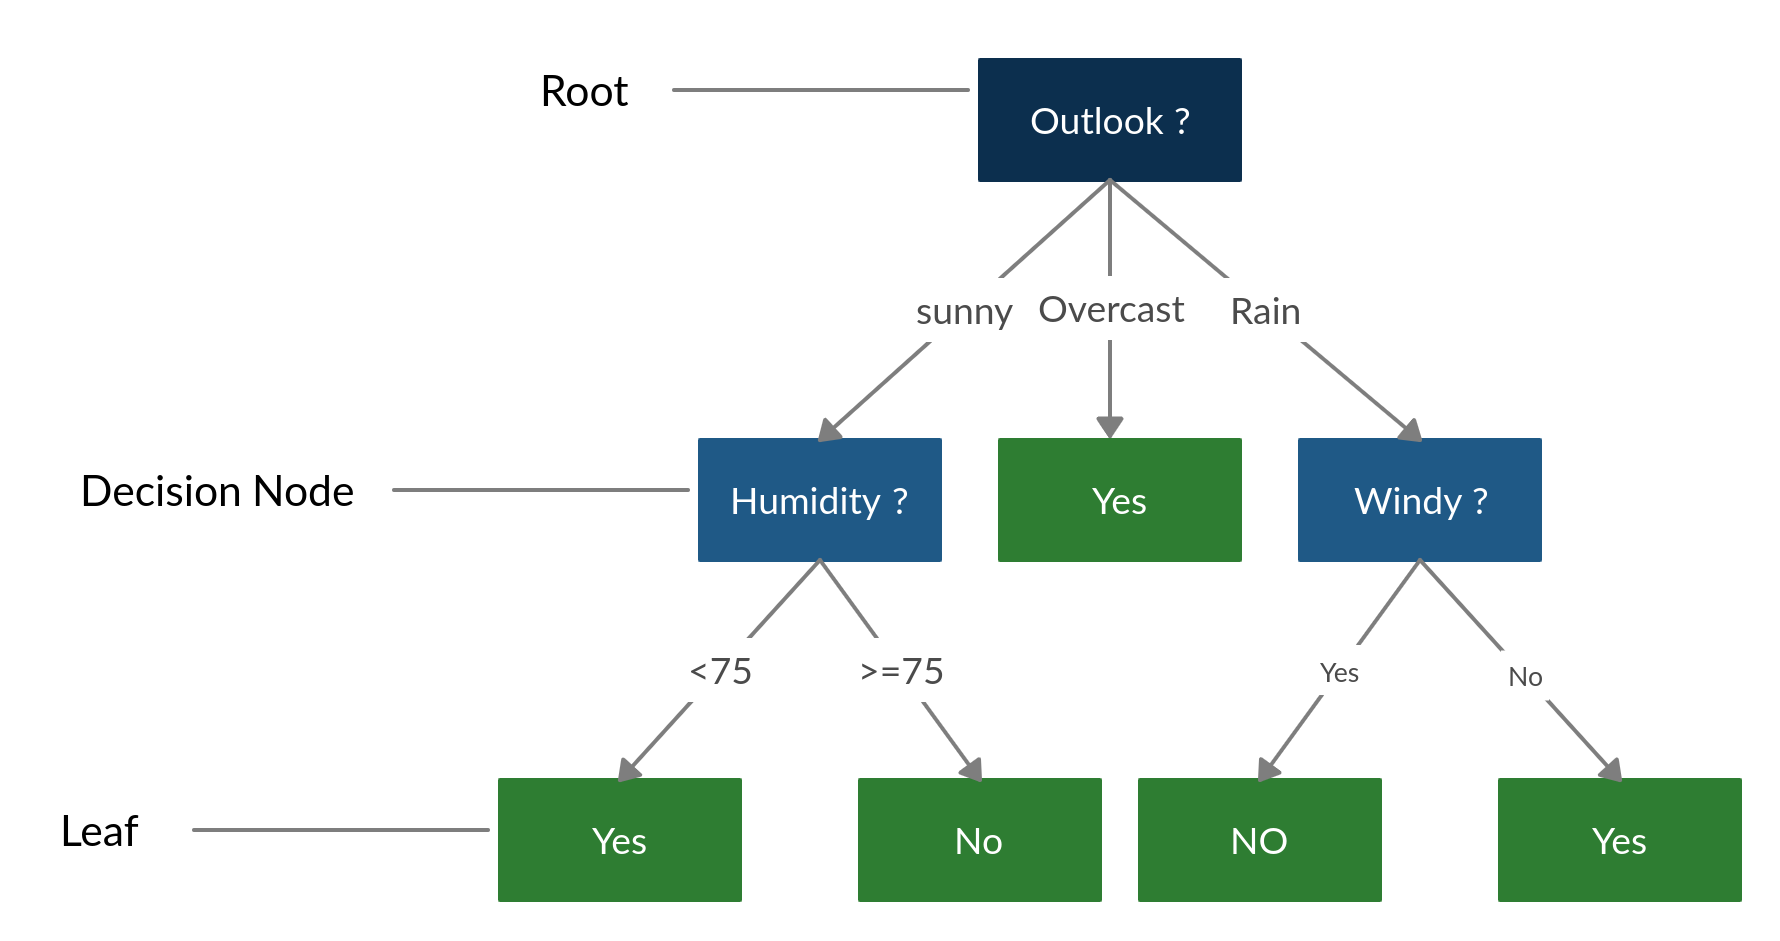
\includegraphics[width=15cm]{Pictures/decision_tres_1.jpg}
    \caption{An example of decision tree.}
    \label{fig:decision_tree}
\end{figure}

The algorithm used to build  DT is called ID3.  J. R. Quinlan developed a top-down, greedy search through the space of possible branches with no backtracking approach has been used in this algorithm . ID3 uses Entropy (equation \ref{entropy} )and Information Gain (equation \ref{gain}) to split a set to subsets,while constructing  a decision tree.
\paragraph{Entropy} : measure of randomness
\begin{equation}
    E(S)=\sum_{i=1}^c -p_i log_2 p_i
    \label{entropy}
\end{equation}
Here,\\
S:class name\\
c: types of values (2 for binary ) \\
$p_i$ : count of values of $i^{th}$ type\\
\paragraph{Gain} : gain in entropy after splitting in to subsets
    \begin{equation}
        G(T,X) = E(T) - E(T,X)
        \label{gain}
    \end{equation}
An illustrative example has been shown in Figure \ref{fig:decision_tree}.In the Figure \ref{fig:decision_tree} if the outlook is sunny then we predict on the basis of  humidity,if it is rainy then we check the wind.   
\subsection{Gradient Boosting Classifier}

It is an ML model for classification and regression problems, in which a prediction model has to be constructed in the form of a combination of weak prediction models, typically decision trees used as a week prediction model.Like other boosting methods do gradient boosting algorithm also builds the model in a stage-wise fashion , and to generalize them it allow optimization of an arbitrary differentiable loss function.

% \subsection{Perceptron}

\subsection{XgBoost}
XGBoost is the leading model for working with standard tabular data.To reach peak accuracy, XGBoost models require more knowledge and model tuning than techniques like Random Forest.XGBoost is an implementation of the Gradient Boosted Decision Trees algorithm.Figure \ref{fig:xg_boost} shows a flow diagram of xgBoost.
\begin{figure}
    \centering
    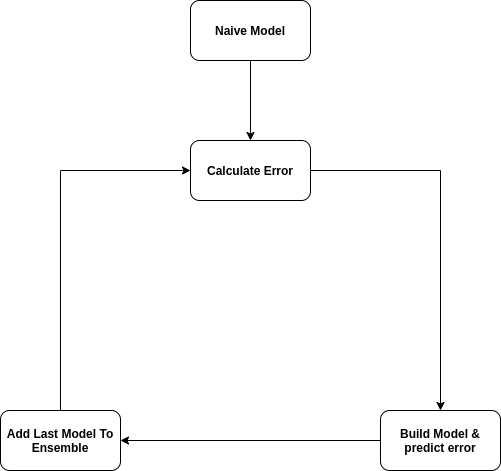
\includegraphics[width=10cm]{Pictures/xgboost.png}
    \caption{XgBoost Flow Chart}
    \label{fig:xg_boost}
\end{figure}

\subsection{Random Forest}
Random forest is a bootstrapping algorithm which uses Decision tree classifier.In our case there is 977 observations with 3328 attribute each.With different initial variables ad different samples, Random forest tries to build multiple decision tree models . For instance, it will build a decision model with a random sample of 100 observation and 5 randomly chosen initial variables. To  make a final prediction, it repeats the process (say) 10 times on every instance. The final prediction is the return of a function which operates on each prediction. We can just take the mean of all the prediction to give final prediction.In Figure \ref{fig:random_forest} we have shown diagram of random forest processing.


\begin{figure}[ht]
    \centering
    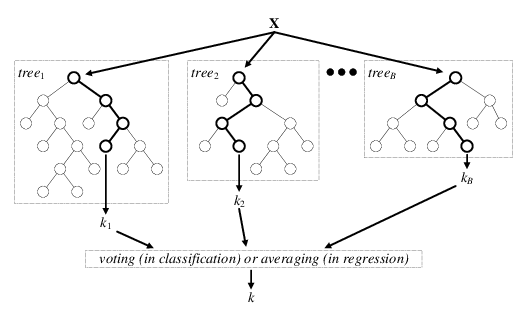
\includegraphics[width=15cm]{Pictures/random_forest_1.png}
    \caption{Random Forest diagram }
    \label{fig:random_forest}
\end{figure}


In the Figure \ref{fig:random_forest},the final prediction will be the value obtained by using voting or averaging method on the predictions of $tree_1$, $tree_2$ ... $tree_B$ i.e. the $k_1,k_2$ and $k_3$. 